

\setcounter{chapter}{10-1} %Makes the prereq chapter chapter 0

\chapter{Recurrent Neural Networks}

    \subsection{Review: Neural Networks So Far}

        In this class, we have built up some powerful tools, and built them into \textbf{models} we can teach to handle different tasks.
        
        All of this has culminated in the \textbf{neural network}: a class of models that can handle a huge number of interesting problems.
        
            \begin{itemize}
                \item All we had to do was combine many simple models together in a systematic, \textbf{nonlinear} way!
                    \note{Remember that by "systematic", we mostly just mean "organized": that way, we can do math easier!}
            \end{itemize}
        
        We then discovered a \textit{weakness} of neural networks: they don't understand \textbf{space} very well! 
            \begin{itemize}
                \item Our models had trouble recognizing that pixels in an image close to each other were more \textit{related} than pixels far away, for example.
            \end{itemize}
            
        The solution was the \textbf{convolutional} neural network: we used \textit{convolution} as a way to represent which elements were "near" each other in space.
        
    \secdiv
        
    \subsection{Time in a Neural Network}
    
        If we want our models to be able to handle \textit{space}, we might also wonder: can we make it so they understand \textbf{time} as well?
        
        Right now, our neural networks have no built-in way to represent \textit{time}: each data point stands by itself.
            \note{Note that we're focused on the finished model: sure, time passes while training, but the final model doesn't keep track of the past.}
            
        For example, suppose we have two data points $\ex{x}{1}$ and $\ex{x}{2}$. To our current neural network, there's \textbf{no difference} if we \textbf{switched} the order of those data points.
        
        But what if it \textit{does} matter? In real life, past information can matter a lot, as can the order.
        
        \miniex If you injured your leg yesterday, you probably don't want to walk around on it too much today. If you injured it a month ago, you might not care.\\
        
        \begin{concept}
            A traditional \vocab{neural network} cannot easily use information about \vocab{time}, or the \purp{past}.
        \end{concept}
        
    \secdiv
        
    \subsection{Our plan going forward}
        
        Now that we've settled on approaching the problem of \textbf{time}, we'll spend the next couple chapters building ways to tackle this problem:
        
        \begin{itemize}
            \item \textbf{Ch.9:} First, we'll build something called a "\textbf{state machine}" to record information about time.
                \begin{itemize}
                    \item We'll use this "machine" to modify our neural networks, creating something called a \textbf{recurrent neural network} (RNN) that can analyze information over time.
                \end{itemize}
            
            \item \textbf{Ch.10:} Then, we'll create a model that makes \textbf{decisions} over time: a "\textbf{Markov Decision Process}" (MDP).
            
            \item \textbf{Ch.11:} Finally, we'll use state machines to \textbf{learn} how to make good decisions in an unknown environment: this is \textbf{Reinforcement Learning}.
        \end{itemize}

\pagebreak

\section{State Machines}

    \subsection{Possible ways to model time}

        We said that we want to think about time, but what does that really mean?
        
        \miniex In the simplest case, we'd just keep track of the \textit{current} timestep $t$.
        
        This is too \textit{little} information. It doesn't really tell us that much: if I told you "the current time is $t=1563$", that doesn't help you make decisions without more context.
        
        Let's use the \textit{injured leg} example: 
        
        \miniex If you injured your leg yesterday, we might want to remember the \textbf{event}, and when the event \textbf{happened}. 
        
        But eventually, your leg \textit{heals}, and that event doesn't \textbf{matter} anymore. As time continues, we'd gather more and more events... that could get \textbf{expensive} to keep track of.
        
        So, remembering every event is too \textbf{much} information.
        
    \secdiv
    
    \subsection{States}
    
        At this point, someone might get annoyed: "just tell me whether my leg hurts or not!" And therein lies our solution.
        
        \miniex The only information we care about is the current \textbf{state} of your leg: is it injured or is it not?
        
        Thus, we only store information about our current condition that \textbf{matters}: we need to update this over time, of course.
        
        This is called a \textbf{state}.\\
        
        \begin{definition}
            A \vocab{state} is some information we use to keep track of the \purp{current situation} you're in.
            
            A state allows us to keep some "\gren{memory}" of the past, but only the parts that matter:
            
            If an event has \purp{changed} the situation, it'll change the \vocab{state}.
            
            A state can be almost \purp{any information} that we want to keep. It can contain \gren{multiple} different pieces of information, as well.
        \end{definition}
        
        \miniex Suppose that you're an investor. Your state could include: 1. how much money you have, 2. the stocks you current own, and 3. whether the market seems to be going up or down.
        
        Notice that, while these variables don't give you exact time, they do \textbf{remember} past events: if you have $\$30$, you at some point must have gotten those $\$30$.
        
        There are many other kinds of states: position and velocity of an object, or the progress on a project, etc.
        
        \subsecdiv
        
        \subsubsection{How states are stored}
    
            Now, we want to know how to notate this consistently:\\
            
            \begin{notation}
                Typically, a \vocab{state} \red{$s$} stores our information.
                
                We represent the \redd{set} of all \redd{states} as \red{$\mathcal{S}$}. 
                
                \begin{itemize}
                    \item We can have a \textbf{finite} or \textbf{infinite} set of states, depending on the situation.
                    \item Since $\mathcal{S}$ contains all of our states, we can say \red{$s \in S$}.
                \end{itemize}
                
                Our state at time $t$ is \red{$s_t$}.
                
                Our \vocab{initial state} ($t=0$) is represented as \red{$s_0$}.         
                \begin{itemize}
                    \item Since it's a state, $s_0 \in \mathcal{S}$.
                \end{itemize}
            \end{notation}
            
            We now have two of the pieces of our state machine:
            
            \begin{itemize}
                \item $\red{\mathcal{S}}$ is a finite or infinite \textbf{set} of possible \textbf{states} \red{$s$}.
                \item $\red{s_0 \in \mathcal{S}}$ is the \textbf{initial state} of the machine. 
            \end{itemize}
        
        \subsecdiv
        
        \subsubsection{State examples}
            Let's show a couple examples of what states different systems might have.
                \note{There are multiple different ways to represent the same set of states with a vector, so we won't specify that representation.}
            
            \begin{itemize}
                \item The game of chess.
                    \begin{itemize}
                        \item The \textbf{finite} set \red{$S$} is the set containing \red{every chess board}.
                        \item The initial state \blu{$s_0$} is the \blu{board} when you first \blu{start playing}.
                    \end{itemize}
                    
                \item A ball moving in space, with coordinates.
                    \begin{itemize}
                        \item The \textbf{infinite} set \red{$S$} contains \red{every pair $[\text{position},\text{velocity}]$} for the ball.
                            \begin{itemize}
                                \item For example, the ball might be:
                                \item at position $(1,2)$, 
                                \item with velocity $(5,0)$.
                                
                            \end{itemize}
                        \item The initial state \blu{$s_0$} is the \blu{position and velocity} when you first \blu{release} the ball.
                    \end{itemize}
                    
                \item A combination lock with 3 digits.
                    \begin{itemize}
                        \item The \textbf{finite} set \red{$S$} contains every \red{sequence of 3 digits}, where only one sequence unlocks the lock.
                            \begin{itemize}
                                \item For example: $[0,0,0]$, \; $[4,6,9]$, \; $[9, 0, 2]$, \; etc.
                            \end{itemize}
                        \item The initial state \blu{$s_0$} is the \blu{sequence} when you \blu{leave} your lock; maybe $[1,2,3]$.
                    \end{itemize}
            \end{itemize}
    
    \subsection{Inputs and Transitions}
    
        We now have a way to \textbf{store} our information in time. However, we need to know how to \textbf{update} our state: what happens if we learn new information? 
        
        In order to do this, we'll create a few more variables. 
        
        \subsubsection{Input}
            First, we get some kind of \textbf{input} $x$, which is our update: this is the most recent information we have. This is \textit{also} stored in a vector.\\
            
            \begin{definition}
                The \vocab{input} \org{$x$} represents \purp{new information} we get from our system.
                
                We represent the \org{set} of all possible \org{inputs} as \org{$\mathcal{X}$}.
                    \begin{itemize}
                        \item This set can be \textbf{finite} or \textbf{infinite}.
                        \item We can say \org{$x \in \mathcal{X}$}.
                    \end{itemize}
                    
                Our input at time $t$ is \org{$x_t$}.
            \end{definition}
            
        \subsecdiv
                
        \subsubsection{Transition}
            
            Now, how do we use this input? Well, our new information will affect our \textbf{state}. But, often, \textbf{how} it affects our state depends on the state itself.
            
            \miniex Suppose you're taking care of a plant.
            
            \begin{itemize}
                \item If a plant is dry ($s_t=$ Dry), then watering it will make it healthier ($s_{t+1}=$ Healthy).
                \item If the plant is watered ($s_t=$ Healthy), then watering it more might make it sick ($s_{t+1}=$ Sick).
            \end{itemize}
            
            We're \textbf{transitioning} between states, so we use a \textbf{transition function}.\\
            
            \begin{definition}
                The \vocab{transition function} \gren{$f_s$} tells us how to update our \red{state}, based on our new \org{input} information.
                
                Thus, our transition takes in two pieces of information: \red{$s$} and \org{$x$}.
                
                \begin{equation*}
                    \grn{f_s}(\red{s},\org{x})
                \end{equation*}
                
                We use this function at every timestep $t$ to get our next state, at time $t+1$.
                
                \begin{equation*}
                    \grn{f_s}(\red{s_t},\org{x_t}) = \red{s_{t+1}}
                \end{equation*}
                
                We can treat each state-input pair as an object, $(s,x)$. Thus, the set of all of these pairs is $\mathcal{S} \cross \mathcal{X}$.
                
                \begin{equation*}
                    \grn{f_s}: \red{\mathcal{S}} \cross \org{\mathcal{X}} 
                    \rightarrow \red{\mathcal{S}}
                \end{equation*}
            \end{definition}
            
            We can visualize this as:
            
            \begin{equation}
                \begin{matrix}
                    \text{\red{State}} \\
                    \text{\org{Input}}
                \end{matrix}
                \longrightarrow
                \boxed{\grn{f_s}}
                \longrightarrow
                \text{\red{New state}}
            \end{equation}
                
            Now, we have two more pieces of our state machine:
            
            \begin{itemize}
                \item \org{$\mathcal{X}$} is a finite or infinite set of possible \textbf{inputs} \org{$x$}.
                \item \grn{$f_s$} is the \textbf{transition function}, which moves us from one state to the next, based on the input.
                    \begin{equation}
                        \grn{f_s}: \red{\mathcal{S}} \cross \org{\mathcal{X}} 
                        \rightarrow \red{\mathcal{S}}
                    \end{equation}
            \end{itemize}
        
        \subsubsection{Transition Examples}
        
            Now, we revisit our examples, and consider how they "transition":
            
            \begin{itemize}
                \item The game of chess.
                    \begin{itemize}
                        \item The input \org{$x$} is the \org{choice} our player makes, \org{moving one piece} on the chess board according to the \textbf{rules}.
                        
                        \item The transition function \grn{$f_s$} applies this move to our current chess board, and produces a \grn{new chess board}.
                            \begin{itemize}
                                \item If we moved our pawn, the transition function outputs the board \grn{after} that pawn is \grn{moved}.
                            \end{itemize}
                    \end{itemize}
                    
                \item A ball moving in space, with coordinates.
                    \begin{itemize}
                        \item The input \org{$x$} might represent a \org{push} changing the ball's velocity.
                        
                        \item The transition function \grn{$f_s$} uses the push to change our \org{velocity}, and the velocity to change the ball's \org{position}.
                            \begin{itemize}
                                \item If our ball wasn't moving before, and we \grn{push} it, the new state is \grn{moving} in that direction.
                            \end{itemize}
                    \end{itemize}
                    
                \item A combination lock with 3 digits.
                    \begin{itemize}
                        \item The input \org{$x$} is you \org{changing} one of the three digits on the lock: for example, \org{increasing} the first digit by 3.
                        
                        \item The transition function \grn{$f_s$} applies the \grn{change} you make to the lock.
                            \begin{itemize}
                                \item If the first digit was \2, and you \grn{increase} it by 3, the new first digit is 5.
                            \end{itemize}
                    \end{itemize}
            \end{itemize}
        
    \secdiv

    \subsection{Output and Output Function}
    
        We now have a system for keeping \textbf{track} of our state, and \textbf{updating} that state: this is a really powerful tool for managing time!
        
        We're still missing something, though: why do we \textbf{care} about our state? We should have some sort of \textbf{reason} for wanting to store the state. 
        
        \subsubsection{Output}
        
            Usually, that information is more simple than all of the parts of the state we want to \textbf{remember}.
            
            \miniex In the above case, where we wanted to know if our leg was injured, the real thing we cared about was: \textbf{can I walk or not}?
            
            The is what we call our \textbf{output}.\\
            
            \begin{definition}
                The \vocab{output} \purp{$y$} represents the \purp{result of our current state}. 
                
                What we consider the "output" often depends on what we are \purp{focused on}.
                
                    \begin{itemize}
                        \item Sometimes, the output is the \textbf{only} thing (aside from input) we can \textbf{see}. This happens when the state is \vocab{hidden}!
                    \end{itemize}
                
                In other words, while the state \textbf{stores} relevant information to keep track of the situation, the \purp{output} is the result of this information.
                
                We represent the \purp{set} of all possible \purp{outputs} as \purp{$\mathcal{Y}$}.
                
                \begin{itemize}
                    \item This set can be \textbf{finite} or \textbf{infinite}.
                    \item We can say \purp{$y \in \mathcal{Y}$}.
                \end{itemize}
                    
                Our output at time $t$ is \purp{$y_t$}.
            \end{definition}

            
        \subsecdiv
        
        \subsubsection{Output Function}
        
            How do we get this output? Well, we use all the information we've \textbf{gathered}. 
            
            We could include both the input and the state, but the state has already been \textbf{updated} to reflect the input. So, we only need that.
            
            This reflects what we said before: our state exists to store \textbf{memory}, and use the information to create an \textbf{output}.
            
            We turn state into the output using an \textbf{output function}.\\
            
            \begin{definition}
                The \vocab{output function} \grn{$f_o$} tells us what \purp{output} we get based on our current \red{state}.
                
                Thus, our \grn{output function} only takes in the \red{state}. 
                
                \begin{equation*}
                    \grn{f_o}(\red{s_t}) = \pur{y_t}
                \end{equation*}
                
                It uses our current information (\red{state}) to produce a new result we're interested in (\purp{output}).
                
                Using sets, we can write this as:
                
                \begin{equation*}
                    \grn{f_o}: \red{\mathcal{S}} \rightarrow \pur{\mathcal{Y}}
                \end{equation*}
            \end{definition}
            
            We visualize this unit as:
            
            \begin{equation*}
                \text{\red{State}} 
                \longrightarrow \boxed{\grn{f_o}} \longrightarrow 
                \text{\purp{Output}}
            \end{equation*}
            
            This gives us the last two parts of our state machine:
            
            \begin{itemize}
                \item \purp{$\mathcal{Y}$} is a finite or infinite set of possible \textbf{outputs} \purp{$y$}.
                
                \item \grn{$f_o$} is an \textbf{output function}, which gives us our output based on our state.
                    \begin{equation}
                        \grn{f_o}: \red{\mathcal{S}} \rightarrow \pur{\mathcal{Y}}
                    \end{equation}
            \end{itemize}
        
        \subsecdiv
        
        \subsubsection{Output Examples}
        
            Again, we go to our examples, and give them outputs, completing our state machines:
            
            \begin{itemize}
                \item The game of chess.
                    \begin{itemize}
                        \item The output \purp{$y$} could be many things. But, what do we care about most: winning! 
                            \begin{itemize}
                                \item So, \purp{$\mathcal{Y}$} will have four options: "ongoing", "draw", "player 1 win", "player 2 win".
                            \end{itemize}
                            
                        \item The output function \grn{$f_o$} will give us our output. Thus, it represents the chess rules for whether there is a winner or a draw.  
                            \begin{itemize}
                                \item So, \grn{$f_o$} looks at a board, and tells us whether someone has won, or there's a draw.
                            \end{itemize}
                    \end{itemize}
                    
                \item A ball moving in space, with coordinates.
                    \begin{itemize}
                        \item The output \purp{$y$} again depends on what we care about.     \begin{itemize}
                                \item Sometimes, the \purp{output} is the same as the \red{state}: all we want to know is what's \red{happening}!
                                \item In this case, we'll say our \textbf{output is the state}: we return the position and velocity of the ball.
                                    \note{We could have chosen a different output if we had a specific goal in mind!}
                            \end{itemize}
                            
                        \item If our state and output are the same, then the output function \grn{$f_o$} shouldn't alter the state it receives!
                            \begin{itemize}
                                \item Our function is the identity: $\grn{f_o}(\red{s}) = \red{s}$.
                            \end{itemize}
                    \end{itemize}
                    
                \item A combination lock with 3 digits.
                    \begin{itemize}
                        \item We want our output \purp{$y$}. 
                            \begin{itemize}
                                \item Our goal is more clear: we want the combination lock to be \textbf{open} or \textbf{closed}. So, those are our outputs \purp{$\mathcal{Y}$}.
                            \end{itemize}
                            
                        \item Our function \grn{$f_o$} will tell us the lock is open if the current digits exactly match the correct sequence.
                    \end{itemize}
            \end{itemize}
    
    \secdiv
    
    \subsection{Our completed State Machine}
    
        Finally, we can assemble our completed state machine.\\
        
        \begin{definition}
            A \vocab{State Machine} can be formally defined as a collection of several objects 
            
            \begin{equation*}
                (\red{\mathcal{S}}, \org{\mathcal{X}}, \pur{\mathcal{Y}}, 
                \red{s_0}, \grn{f_s}, \grn{f_o})
            \end{equation*}
            
            We have three sets:
            
            \begin{itemize}
                \item $\red{\mathcal{S}}$ is a finite or infinite \textbf{set} of possible \textbf{states} \red{$s$}.
                
                \item $\org{\mathcal{X}}$ is a finite or infinite \textbf{set} of possible \textbf{inputs} \org{$x$}.
                
                \item $\pur{\mathcal{Y}}$ is a finite or infinite \textbf{set} of possible \textbf{outputs} \purp{$y$}.
            \end{itemize}
            
            And components to allow us to transition through time:
            
            \begin{itemize}
                \item $\red{s_0 \in \mathcal{S}}$ is the \textbf{initial state} of the machine. 
                
                \item \grn{$f_s$} is the \textbf{transition function}, which moves us from one state to the next, based on the input.
                    \begin{equation*}
                        \grn{f_s}: \red{\mathcal{S}} \times \org{\mathcal{X}}
                        \rightarrow \red{\mathcal{S}}
                    \end{equation*}

                \item \grn{$f_o$} is an \textbf{output function}, which gives us our output based on our state.
                    \begin{equation*}
                        \grn{f_o}: \red{\mathcal{S}} \rightarrow \pur{\mathcal{Y}}
                    \end{equation*}
            \end{itemize}
        \end{definition}
        
        We have:
        
        \begin{itemize}
            \item Our \textbf{state} to preserve information,
            \item Our \textbf{input} to update information,
            \item Our \textbf{output} gives us the result of our information.
        \end{itemize}
        
        And to combine these, we need:
        
        \begin{itemize}
            \item Our \textbf{initial} state,
            \item How to \textbf{change} states,
            \item How to \textbf{get} an \textbf{output}.
        \end{itemize}
    
    \secdiv
    
    \subsection{How to use a state machine}
    
        How do we work with a state machine? Well, we have all of the tools we need.
        
        We start with out initial state, $\red{s_0}$. For our \textbf{first} timestep, we get a new input: new \textbf{information}. We use this to get a new state.
        
        \begin{equation}
            \red{s_1} = 
            \grn{f_s}(\red{s_0}, \org{x_1})
        \end{equation}
        
        With this state, we can now get our \textbf{output}.
        
        \begin{equation}
            \pur{y_1} = 
            \grn{f_0}(\red{s_1})
        \end{equation}
        
        We've calculated everything in our \textbf{first} timestep! Now, we can move on to our \textbf{second} timestep, and do the same thing.
        
        In general, we'll repeatedly follow the process:
        
        \begin{equation}
            \red{s_t} = 
            \grn{f_s}(\red{s_{t-1}}, \org{x_t})
        \end{equation}
        
        \begin{equation}
            \pur{y_t} = 
            \grn{f_o}(\red{s_t})
        \end{equation}
        
        
        \begin{concept}
            To move through time in a state machine, we follow these steps from $t=1$:
            
            \begin{itemize}
                \item Use the \org{input} and \red{state} to get our \red{new state}.
                    \begin{equation*}
                        \red{s_t} = 
                        \grn{f_s}(\red{s_{t-1}}, \org{x_t})
                    \end{equation*}
                    
                \item Use the \red{new state} to get our \pur{output}.
                    \begin{equation*}
                        \pur{y_t} = 
                        \grn{f_o}(\red{s_t})
                    \end{equation*}
                    
                \item Increment the time from $t$ to $t+1$.
                
                    \begin{equation*}
                        t_{new} = t_{old} + 1
                    \end{equation*}
                
                \item Repeat.
            \end{itemize}
        \end{concept}
        
        \subsecdiv
        
        \subsubsection{Example of State Machine}
        
            To make this more concrete, we'll build our own simple state machine and run a couple iteration steps.
                
            Suppose you're saving up money to buy something. At each timestep, you gain or lose some money. 
            
            You want to know when you have enough money to buy it. 
                \note{This example is simple enough that you might feel like a state machine is unnecessary. However, this is just for demonstration!}
                
            What are each of the parts of our state machine?
            
            \begin{itemize}
                \item The state $\red{s}$: how much money do we have right now?
                
                \item The input $\org{x}$: the money we add to our savings.
                
                \item The output $\pur{y}$: we want to know when we have enough money. Maybe our goal is 10 dollars.
                
                \item Initial $\red{s_0}$: we start with 0 dollars.
                
                \item Transition $\grn{f_s}$: we just add the new money to how much we have saved up.
                
                    \begin{equation}
                        f_s(\red{s},\org{x}) = \red{s}+\org{x}
                    \end{equation}
                    
                \item Output $\grn{f_o}$: do we have enough money?
                
                    \begin{equation}
                        \grn{f_o}(\red{s}) = (\red{s} \geq 10)
                        =
                        \begin{cases}
                            \text{True} & \text{If } s \geq 10 \\
                            \text{False} & \text{Otherwise}
                        \end{cases}
                    \end{equation}
            \end{itemize}
            
            We'll run through our state machine for the following input:
            
            \begin{equation}
                \red{X} = [x_1, \; x_2, \; x_3, \; x_4] = [ 4, \; 5, \; 6, \; -7]
            \end{equation}
            
            Let's apply the steps above:
            
            \begin{itemize}
                \item Get new state from (old state, input).
                \item Get output from new state.
                \item Increment time counter.
            \end{itemize}
            
            For our first step, we get:
            
            \begin{equation}
                \begin{matrix}
                    \red{s_1} = 4+0 = \red{4} \\
                    \\
                    \pur{y_1} = ( 4 \geq 10 ) = \text{\pur{False}}
                \end{matrix}
            \end{equation}
            
            For the others, we get:
            
            \begin{equation}
                \begin{matrix}
                    \red{s_2} = 9 \\ \pur{y_2} = \text{False}
                \end{matrix}
                \;\; \longrightarrow \;\; 
                \begin{matrix}
                    \red{s_3} = 15 \\ \pur{y_3} = \text{True}
                \end{matrix}
                \;\; \longrightarrow \;\; 
                \begin{matrix}
                    \red{s_4} = 8 \\ \pur{y_4} = \text{False}
                \end{matrix}
            \end{equation}
            
            Though our transition and output functions might become more complicated, this is the basic idea behind all state machines.
    
    \secdiv 
    
    \subsection{State Machine Diagram}
    
        Finally, we'll create a visualization that represents our state diagram.
        
        \subsubsection{Transition Function}
        
            Our \grn{transition function} follows this format:
            
            \begin{equation}
                \red{s_t} = 
                \grn{f_s}(\red{s_{t-1}}, \org{x_t})
            \end{equation}
            
            We can diagram this component as:
            
            \begin{figure}[H]
                \centering
                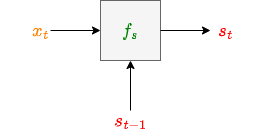
\includegraphics[width=60mm,scale=0.4]{images/rnn_images/transition_diagram.png}
            \end{figure}
            
            Note that the state appears \textbf{twice}: once as an input, once as an output.
            
            In the \textit{next} timestep, $s_t$ will be the \textbf{input} to $f_s$, even though it's currently the \textbf{output}.
                \note{If $t=10$, then $s_{10}$ is the output. If $t=11$, then $s_{10}$ is the input!}
                
            We'll create a way to represent this later.
        
        \subsecdiv
        
        \subsubsection{Output Function}
        
            Our \grn{output function} takes in the state we just got from the transition function:
            
            \begin{equation}
                \pur{y_t} = 
                \grn{f_o}(\red{s_t})
            \end{equation}
            
            So, we diagram it accordingly:
            
            \begin{figure}[H]
                \centering
                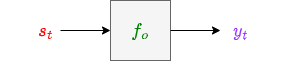
\includegraphics[width=60mm,scale=0.4]{images/rnn_images/output_diagram.png}
            \end{figure}
            
            As we mentioned, the \textbf{output} function takes in the \textbf{transition} function as its input: let's depict that! We'll combine our two units.
            
            \begin{figure}[H]
                \centering
                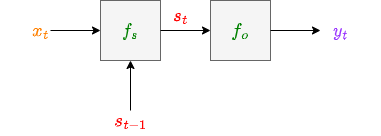
\includegraphics[width=80mm,scale=0.4]{images/rnn_images/state_machine_protodiagram.png}
            \end{figure}
            
        \subsecdiv
        
        \subsubsection{Time Delay}
        
            Only one thing is missing: we know that our current state $\red{s_t}$ needs to be reused \textbf{later}: we'll need it to compute our \textit{new} state $\red{s_{t+1}}$.
            
            We don't want it to \textit{immediately} send the state information back to $f_s$: we only use the function once per timestep. So, we'll \textit{delay} by waiting one time step.
            
            We'll use a little clock symbol to represent this fact.
            
            \begin{figure}[H]
                \centering
                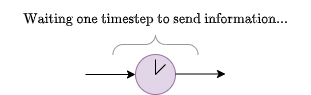
\includegraphics[width=80mm,scale=0.4]{images/rnn_images/clock.png}
            \end{figure}
            
            \begin{notation}
                We can depict a \vocab{state machine} using the following diagram:
                
                \begin{figure}[H]
                    \centering
                    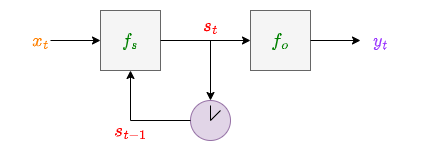
\includegraphics[width=90mm,scale=0.4]{images/rnn_images/state_machine_diagram.png}
                \end{figure}
                
                At every timestep, we use $\org{x_t}$ and $\red{s_{t-1}}$ to calculate our new state, and our new output.
                
                The circular "clock" element represents our \purp{delay}: $\red{s_t}$ becomes the input to $f_s$ on the \purp{next} timestep.
            \end{notation}
    
    \secdiv
    
    \subsection{State Transition Diagrams}
    
        \subsubsection{Finite State Machines}
    
            To get used to state machines, we'll start with a simpler, special case, the \textbf{finite state machine}.\\
            
            \begin{definition}
                A \vocab{finite state machine} is a state machine where
                
                \begin{itemize}
                    \item The set of states $\red{\mathcal{S}}$
                    \item The set of inputs $\org{\mathcal{X}}$
                    \item The set of outputs $\pur{\mathcal{Y}}$
                \end{itemize}
                
                Are all \vocab{finite}. Meaning, the total space of our state machine is \purp{limited}.
                
                Each aspect of our state machine can be put into a finite list of elements: this often makes it easier to \textit{fully} describe our state machine.
            \end{definition}
            
            This seemingly limited tool is more powerful than it seems: \textbf{all computers} can be described as finite state machines!
                \note{Even when a computer seems to be describing "infinite" collections of things, it only has a finite amount of space to represent them.}
                
        \subsecdiv
        
        \subsubsection{State Transition Diagrams}
        
            One nice thing about the simplicity of a finite state machine is that we can represent it \textbf{visually}.
            
            Let's build one up: we'll pick a simple, though not entirely realistic example.
            
            We have a blanket. It can be in three states: either \blu{wet}, \grn{dry}, or \red{burning}. We can represent each state as a "node".
            
            \begin{figure}[H]
                \centering
                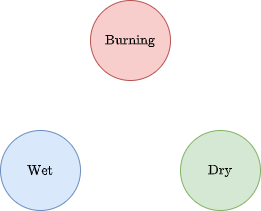
\includegraphics[width=60mm,scale=0.4]{images/rnn_images/std_states.png}
            \end{figure}
            
            \begin{concept}
                In a \vocab{state transition diagram}, states are represented as \purp{nodes}, or points on the graph.
            \end{concept}
            
            We have our states down. The other important thing is our \textbf{transitions}. How do we go between states?
            
            Well, one input could be \textbf{water}: it would stop the blanket from burning. In any case, the blanket will be wet.
            
            \begin{figure}[H]
                \centering
                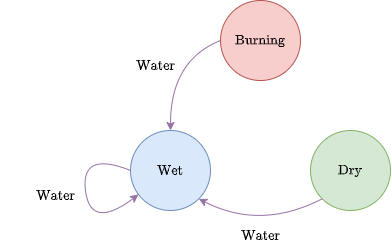
\includegraphics[width=80mm,scale=0.4]{images/rnn_images/std_water.png}
            \end{figure}
            
            Now, we can see: each arrow represents a \textbf{transition} between two states. Each \textbf{input} gets its own transition.\\
            
            \begin{concept}
                In a \vocab{state transition diagram}, transitions are represented as \purp{arrows} between states.
                
                We usually label these with whichever \org{input} will cause that transition.
            \end{concept}
            
            Also notice that a state can transition to itself: a wet blanket \textbf{stays wet} when you add water.
            
            What if we add \textbf{fire}? That would make a dry blanket \textbf{burn}. But, we could also use it to \textbf{dry off} the wet blanket!
            
            \begin{figure}[H]
                \centering
                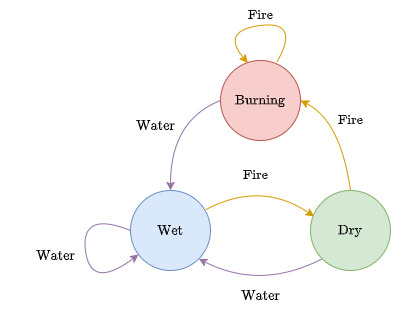
\includegraphics[width=80mm,scale=0.4]{images/rnn_images/std_fire_and_water.png}
            \end{figure}
            
            And now, we have a simple \textbf{state transition diagram}!
                \note{Note that our diagram doesn't have to show the output: the output is given by the state, so each node has its own output}
            
            Each transition, as usual, is based on two things: the \textbf{current} state (where the arrow starts) and the \textbf{input}(which arrow you follow).\\
            
            \begin{definition}
                A \vocab{state transition diagram} is a \purp{graph} of 
                
                \begin{itemize}
                    \item Nodes (\red{points}) representing \red{states}
                    \item Directed edges (\grn{arrows}) representing \grn{transitions}
                \end{itemize}
                
                Where each input-state pair has one arrow associated with it.
                
                These arrows show one \grn{transition}, with the properties:
                
                \begin{itemize}
                    \item The start and end \red{states} represented by the start and the end of the arrow
                    \item The \org{input} that causes this transition is labelled.
                \end{itemize}
                
                This diagram does not have to show the input.
            \end{definition}
            
                \note{If you're not familiar with "nodes" or "edges", don't worry about it! For our purposes, "point" and "arrow" are good enough.}
            
        \subsecdiv
        
        \subsubsection{Simplifying state transition diagrams: one-input graphs}
            
            One more consideration: the graph above is helpful, but it's a bit \textbf{complicated}. 
            
            In fact, if we added more \textbf{states}, or more \textbf{inputs}, it could get too complicated to read!
            
            Our solution: if a system is too complicated, we create a separate state-transition diagram for \textbf{each input}.
            
            \begin{figure}[H]
                \centering
                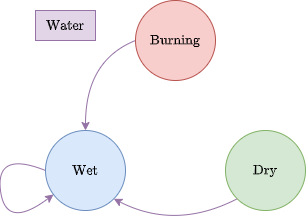
\includegraphics[width=60mm,scale=0.4]{images/rnn_images/std_water_no_label.png}
                \qquad
                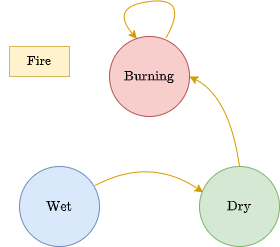
\includegraphics[width=55mm,scale=0.4]{images/rnn_images/std_fire.png}
                
                \caption*{The left diagram only uses \textbf{water} as an input, while the right diagram only uses \textbf{fire} as an input.}
            \end{figure}
            
            Each of our diagrams is much more readable now! Not only do we have less arrows, but we don't have to label each arrow.
            
            As a tradeoff, we have two graphs to keep track of, instead of one. However, this is usually necessary.
                \note{In the next chapter, MDPs, we'll need this!}\\
                
            \begin{concept}
                We can simplify our \vocab{state transition diagrams} by creating a \purp{separate diagram} for each \org{input}.
                
                This makes it easier to visualize what's going on.
            \end{concept}
\section{Recurrent Neural Networks}    
            
            
        
        
        
        

\section{Old Materials}


%%%%%%%%%%%%%%%%%%%%%%%%%%%%%%%%%%%%%%%%%%%%%%%%%%%%%%%%%%%%%%%%%%%%%%%%%%%%%
\section{State machines}
\label{sec:state_machines}


Another common structure that is simple but powerful and used in
signal processing and control is {\em linear time-invariant (LTI)
  systems}\index{linear time-invariant systems}.  In this case, all
the quantities are real-valued vectors: $\mathcal S = \R^m$, $\mathcal
X = \R^l$ and $\mathcal Y = \R^n$. The functions $f_s$ and $f_o$ are
linear functions of their inputs. 
The transition function is described by the state matrix $A$ and the input matrix $B$; 
the output function is defined by the output matrix $C$, each with compatible dimensions.
In discrete time, they can be
defined by a linear difference equation, like
\begin{align}
 s_t &= f_s(s_{t-1}, x_t) = A s_{t-1} + B x_t, \\
 y_t &= f_o(s_t) = C s_t, \;\;
\end{align}
and can be implemented using state to store relevant previous
input and output information.
We will study {\it{recurrent neural networks}} which are a lot like a
non-linear version of an LTI system.

    


%%%%%%%%%%%%%%%%%%%%%%%%%%%%%%%%%%%%%%%%%%%%%%%%%%%%%%%%%%%%%%%%%%%%%%%%%%%%%
\section{Recurrent neural networks}
\label{sec:rnn_model}

In Chapter~\ref{chap:neural_networks}, we studied neural networks and
how the weights of a network can be obtained by training on data, so
that the neural network will model a function that approximates the
relationship between the $(x, y)$ pairs in a supervised-learning
training set.  In Section~\ref{sec:state_machines} above, we
introduced state machines to describe sequential temporal
behavior. Here in Section~\ref{sec:rnn_model}, we explore recurrent
neural networks by defining the architecture and weight matrices in a
neural network to enable modeling of such state machines.  Then, in
Section~\ref{sec:seq2seq_rnn}, we present a loss function that may be
employed for training {\em sequence to sequence} {\sc rnn}s, and then
consider application to language translation and recognition in
Section~\ref{sec:language}.  In Section~\ref{sec:bptt}, we'll see how
to use gradient-descent methods to train the weights of an {\sc rnn}
so that it performs a {\em transduction} that matches as closely as
possible a training set of input-output {\em sequences}.





\section{Sequence-to-Sequence Recurrent Neural Networks}
    \label{sec:seq2seq_rnn}
    
    Recurrent Neural Networks (RNNs) are a powerful tool for modeling sequential data. In this section, we will explore how we can use RNNs to model a specific type of sequential data called sequence-to-sequence mapping.
    
    Sequence-to-sequence mapping is a problem where we are given an input sequence, and we want to learn to generate the corresponding output sequence. This is similar to a regression problem, where we want to learn a function that maps input sequences to output sequences.
    
    In order to train an RNN to perform sequence-to-sequence mapping, we need a training set that consists of input-output sequence pairs. The training set is typically of the form ${(x^{(1)}, y^{(1)}), \dots, (x^{(q)}, y^{(q)})}$, where $x^{(i)}$ and $y^{(i)}$ are sequences of the same length, and sequences in different pairs may have different lengths.
    
    We also need to define a loss function that measures how well the RNN is performing at mapping input sequences to output sequences. One common choice is to sum up a per-element loss function for each output value, where $g$ is the predicted sequence and $y$ is the actual sequence:
    
    \begin{equation}
    \mathcal{L}{\text{seq}}\left(g^{(i)}, y^{(i)}\right) = \sum{t = 1}^{n^{(i)}}\mathcal{L}_\text{elt}\left(g_t^{(i)}, y_t^{(i)}\right)
    \end{equation}
    
    The per-element loss function $\mathcal{L}_\text{elt}$ will depend on the type of $y_t$ and what information it is encoding. A common choice is the negative log-likelihood (NLL) loss function.
    
    The overall goal is to minimize the objective function $J(W)$, where $W$ are the weights of the RNN, and $\text{RNN}(x; W)$ is the output sequence generated by the RNN given input sequence $x$:
    
    \begin{equation}
    J(W) = \frac{1}{q} \sum_{i = 1}^q\mathcal{L}_{\text{seq}}\left( \text{RNN}(x^{(i)};W), y^{(i)}\right)
    \end{equation}
    
    It is common to choose the activation function $f_s$ to be the hyperbolic tangent (tanh) function, which is a non-linear activation function that ranges from -1 to 1. The choice of activation function $f$

    \subsection{Back-propagation through time}
        \label{sec:bptt}
        
        In this section, we will discuss the method of back-propagation through time ({\sc bptt}) which is used to find the optimal values of $W$ that minimizes $J$ using gradient descent. Although, it is not the best method to use, it is relatively easy to understand. In section~lstm, we will discuss alternative methods that are more commonly used.
        
        \begin{concept}
        By "unrolling" a recurrent network out to model a particular sequence, we can treat the whole thing as a feed-forward network with a lot of parameter sharing. Thus, we can tune the parameters using stochastic gradient descent, and learn to model sequential maps. The concepts presented in this section are very important. While the details are important to get right if you need to implement something, the mathematical details are presented primarily to convey the larger concepts.
        \end{concept}
        
    \subsection{Calculus Reminder: Total Derivative}
    
    It is important to understand the difference between the \vocab{partial derivative} and the \vocab{total derivative}. To illustrate this difference, we will use an example from the Wikipedia article on partial derivatives.
    
    Consider the volume of a circular cone, which depends on its height, $h$, and radius, $r$:
    
    \begin{equation*}
    V(r, h) = \frac{\pi r^2 h}{3}
    \end{equation*}
    
    The partial derivatives of the volume with respect to the height and radius are:
    
    \begin{equation*}
    \frac{\partial V}{\partial r} = \frac{2\pi r h}{3}\;\;\;\text{and}\;\;\;
    \frac{\partial V}{\partial h} = \frac{\pi r^2}{3}
    \end{equation*}
    
    These derivatives measure the change in $V$ assuming everything is held constant except the single variable we are changing.
    
    Now, assume that we want to preserve the cone's proportions, such that the ratio of radius to height stays constant. In this case, we must consider the \vocab{total derivative}.
    
    If we are interested in the total derivative with respect to $r$, we sum the paths along which $r$ might influence $V$:
    
    \begin{align*}
    \frac{dV}{dr} & = \frac{\partial V}{\partial r} + \frac{\partial V}{\partial h} \frac{dh}{dr} 
     = \frac{2 \pi r h}{3} + \frac{\pi r^2}{3} \frac{dh}{dr}
    \end{align*}
    
    Alternatively, if we are interested in the total derivative with respect to $h$, we consider how $h$ might influence $V$, either directly or via $r$:
    
    \begin{align*}
    \frac{dV}{dh} & = \frac{\partial V}{\partial h} + \frac{\partial V}{\partial r} \frac{dr}{dh} \
    & = \frac{\pi r^2}{3} + \frac{2 \pi r h}{3} \frac{dr}{dh}
    \end{align*}
    
    To be concrete, let's consider a right circular cone with a fixed angle $\alpha = \tan r / h$, such that if we change $r$ or $h$, then $\alpha$ remains constant. Thus, we have $r = h \tan^{-1} \alpha$ and let constant $c = \tan^{-1} \alpha$, so now $r = c h$. This gives us the final form of the total derivatives:
    
    \begin{align*}
    \frac{dV}{dr} & = \frac{2 \pi r h}{3} + \frac{\pi r^2}{3} \frac{1}{c} \
    \frac{dV}{dh} & = \frac{\pi r^2}{3} + \frac{2 \pi r h}{3} c ; .
    \end{align*}
    















    
\section{END}






    

\bigskip


A {\it recurrent neural network}\index{recurrent neural network} is a state machine with neural
networks constituting functions $f_s$ and $f_o$:
\begin{align}
  s_t & = f_s\left(W^{sx}x_t + W^{ss}s_{t - 1} + W^{ss}_0\right) \\
  y_t & = f_o\left(W^o s_t + W_0^o\right) \;\;.
\end{align}
\note{We are very sorry!   This course material has evolved from 
  different sources, which used $W^Tx$ in the forward pass for regular
  feedforward NNs and $Wx$ for the forward pass in {\sc rnn}s.  This
  inconsistency  doesn't make any technical difference, but is a
  potential source of confusion.
}
The inputs, states, and outputs are all vector-valued:
\begin{align}
x_t &: \ell \times 1 \\
s_t &: m \times 1 \\
y_t &: v \times 1 \;\;.
\end{align}
The weights in the network,  then,  are
\begin{align}
W^{sx} &:  m \times \ell \\
W^{ss} &: m \times m \\
W^{ss}_0 &: m \times 1 \\
W^{o} &: v \times m \\
W^{o}_0 &: v \times 1 
\end{align}
with activation functions $f_s$  and $f_o$.  

\question{Check dimensions here to be sure it all works out.  Remember
  that we apply $f_s$ and $f_o$ elementwise, unless $f_o$ is a
  softmax activation.}

%%%%%%%%%%%%%%%%%%%%%%%%%%%%%%%%%%%%%%%%%%%%%%%%%%%%%%%%%%%%%%%%%%%%%%%%%%%%%
\section{Sequence-to-sequence RNN}

\label{sec:seq2seq_rnn}

Now, how can we set up an {\sc rnn} to model and be trained to produce
a transduction\index{transduction} of one sequence to another?  This problem is sometimes
called {\em sequence-to-sequence} mapgrng\index{sequence-to-sequence mapgrng}.  You can think of it as a
kind of regression problem: given an input sequence, learn to generate
the corresponding output sequence. \note{One way to think of training
  a sequence {\bf classifier} is to reduce it to a transduction
  problem, where $y_t = 1$ if the sequence $x_1, \ldots, x_t$ is a
  {\em positive} example of the class of sequences and $-1$
  otherwise.}

A training  set has the form 
$\left[\left(x^{(1)}, y^{(1)}\right), \dots, \left(x^{(q)},
    y^{(q)}\right)\right]$, where
\begin{itemize}
\item
$x^{(i)}$ and $y^{(i)}$ are length $n^{(i)}$ sequences; 
\item
sequences in the {\it{same pair}} are the same length; and
sequences in different pairs may have different lengths.
\end{itemize}

Next, we need a loss function.  We start by defining a loss function
on sequences.  There are many possible choices, but usually it makes
sense just to sum up a per-element loss function on each of the output
values, where $g$ is the predicted sequence and $y$ is the actual one: 
\begin{equation}
\mathcal{L}_{\text{seq}}\left(g^{(i)}, y^{(i)}\right) = \sum_{t =
    1}^{n^{(i)}}\mathcal{L}_\text{elt}\left(g_t^{(i)},
    y_t^{(i)}\right) \;\;.
\end{equation} 
The per-element loss function $\mathcal{L}_\text{elt}$\note{So it could be  {\sc nll},
squared loss, etc.} will depend on
the type of $y_t$ 
and what information it is encoding, in the same way as for a
supervised network.

Then, letting $W =\left(W^{sx}, W^{ss}, W^o, W^{ss}_0,
  W_0^o\right)$, our overall goal is to minimize the objective
\begin{equation}
 J(W) = \frac{1}{q} \sum_{i = 1}^q\mathcal{L}_{\text{seq}}\left(
    \text{RNN}(x^{(i)};W), y^{(i)}\right) \;\;,
\end{equation}
where $\text{RNN}(x; W)$ is the output sequence generated, given
input sequence $x$.

It is typical to choose $f_s$ to be {\it tanh} \note{Remember that it
 looks like a sigmoid but ranges from -1 to +1.} but any non-linear
activation function is usable.  We choose  $f_o$ to align with the
types of our outputs and the loss function,  just as we would do in
regular supervised learning.


\section{RNN as a language model}
\label{sec:language}

A {\em language model}\index{language model} is a sequence to sequence {\sc rnn} which is
trained on a character sequence of the form, $c = (c_1, c_2,
\ldots, c_k)$, and is used to predict the next character $c_t, t \leq k$,
given a sequence of the previous $(t-1)$ tokens: \note{A ``token'' is generally a
  character or a word.}
\begin{equation}
c_t = \text{RNN}\left((c_1, c_2, \dots, c_{t - 1}) ; W \right)\;\;
\end{equation} 

We can convert this to a sequence-to-sequence training problem by
constructing a data set of $q$ different $(x, y)$ sequence pairs, where we make up
new special tokens, $\text{start}$ and $\text{end}$, to signal the
beginning and end of the sequence:
\begin{align}
x & = (\langle\text{start}\rangle, c_1, c_2, \ldots, c_k)\\
y & = (c_1, c_2, \dots, \langle\text{end}\rangle) 
\end{align}



%%%%%%%%%%%%%%%%%%%%%%%%%%%%%%%%%%%%%%%%%%%%%%%%%%%%%%%%%%%%%%%%%%%%%%%%%%%%%

% \begin{noticebox}
%   The following material on back-propagation through time
%   (Section~\ref{sec:bptt}) and vanishing gradients and gating
%   mechanisms (Section~\ref{sec:rnn_lstm}) is for your own elucidation.
%   It is not being covered in the Fall 2021 semester of 6.036, and will
%   not be included in the final exam.
% \end{noticebox}

\section{Back-propagation through time}
\label{sec:bptt}

Now the fun begins!  We can now try to find a $W$ to minimize $J$
using gradient descent.  We will work through the simplest method,
{\em back-propagation through time}\index{backpropagation through
  time} ({\sc bptt}), in detail.  This is generally not the best
method to use, but it's relatively easy to understand.  In
Section~\ref{lstm} we will sketch alternative methods that are in much
more common use.

\bigskip 
\begin{noticebox}
  What we want you to take away from this section is that, by
  ``unrolling'' a recurrent network out to model a particular
  sequence, we can treat the whole thing as a feed-forward network
  with a lot of parameter sharing.  Thus, we can tune the parameters
  using stochastic gradient descent, and learn to model sequential
  mapgrngs.  The concepts here are very important.  While the details
  are important to get right if you need to implement something, we
  present the mathematical details below primarily to convey or
  explain the larger concepts.
\end{noticebox}


\begin{examplebox} {\bf Calculus reminder: total derivative} Most of
  us are not very careful about the difference between the {\em
    partial derivative} and the {\em total derivative}\index{total derivative}.  We are going
  to use a nice example from the Wikipedia article on partial
  derivatives to illustrate the difference.

The volume of a circular cone depends on its height and radius:
\begin{equation}
V(r, h) = \frac{\pi r^2 h}{3}\;\;.
\end{equation}
The partial derivatives of volume with respect to height and radius
are
\begin{equation}
\frac{\partial V}{\partial r} = \frac{2\pi r
    h}{3}\;\;\;\text{and}\;\;\; 
\frac{\partial V}{\partial h} = \frac{\pi r^2}{3}\;\;.
\end{equation}
They measure the change in $V$ assuming everything is held constant
except the single variable we are changing.
Now assume that we want to preserve the cone's proportions in the sense that the ratio of radius to height stays constant. 
Then we can't really change one without changing the other.  
In this case, we really have to think about the {\em total derivative}. 
If we're interested in the total derivative with respect to $r$, we sum the ``paths'' along which $r$ might influence $V$:
\begin{align}
\frac{dV}{dr} & = \frac{\partial V}{\partial r} + \frac{\partial
  V}{\partial h} \frac{dh}{dr} \\
& = \frac{2 \pi r h}{3} + \frac{\pi r^2}{3} \frac{dh}{dr} 
\end{align}
Or if we're interested in the total derivative with respect to $h$, we consider how $h$ might influence $V$, either directly or via $r$:
\begin{align}
\frac{dV}{dh} & = \frac{\partial V}{\partial h} + \frac{\partial
  V}{\partial r} \frac{dr}{dh} \\
& = \frac{\pi r^2}{3} + \frac{2 \pi r h}{3} \frac{dr}{dh} 
\end{align}

Just to be completely concrete, let's think of a right circular cone
with a fixed angle $\alpha = \tan r / h$, so that if we change $r$ or
$h$ then $\alpha$ remains constant.  So we have $r = h \tan^{-1}
\alpha$;  let constant $c = \tan^{-1} \alpha$, so now $r = c h$.
Thus, we finally have
\begin{align}
\frac{dV}{dr} & = \frac{2 \pi r h}{3} + \frac{\pi r^2}{3} \frac{1}{c} \\
\frac{dV}{dh} & = \frac{\pi r^2}{3} + \frac{2 \pi r h}{3} c \; .
\end{align}

\end{examplebox}

\noindent The {\sc bptt} process goes like this:
\begin{enumerate}[(1)]
\item
Sample a training pair of  sequences $(x, y)$; let their length be $n$.
\item
``Unroll" the RNN to be length $n$ (picture for $n = 3$ below), and
initialize $s_0$:

Now,  we can see our problem as one of performing what is almost an
ordinary back-propagation training procedure in a feed-forward neural
network, but with the difference that the weight matrices are shared
among the layers.  In many ways, this is similar to what ends up
happening in a convolutional network, except in the conv-net, the
weights are re-used spatially, and here, they are re-used temporally.
\item
Do the {\it forward pass}, to compute the predicted output sequence $g$:
\begin{align}
z_t^1 &= W^{sx}x_t + W^{ss}s_{t - 1} + W^{ss}_0\\
s_t &= f_s(z_t^1)\\
z_t^2 &= W^os_t + W_0^o\\
g_t &= f_o(z_t^2)
\end{align}
\item
Do {\em backward pass} to compute the gradients. For both $W^{ss}$ and
$W^{sx}$ we need to find
\begin{align}
\frac{d \mathcal{L}_\text{seq}(g,y)}{d W} &= \sum_{u = 1}^n\frac{d \mathcal{L}_\text{elt}(g_u, y_u)}{d W} ~~~~~~~~~~~~~~~~~~ \nonumber
\end{align}
Letting $\mathcal{L}_u = \mathcal{L}_\text{elt}(g_u, y_u)$ and using the {\em  total derivative}, which is a sum over all
the ways in which $W$ affects $\mathcal{L}_u$, we have
\begin{align}
~~~~ &= \sum_{u = 1}^n\sum_{t = 1}^n  \frac{\partial s_t}{\partial W} \frac{\partial \mathcal{L}_u}{\partial s_t}  \nonumber
\end{align}
Re-organizing, we have
\begin{align}
~~~~ &= \sum_{t = 1}^n\frac{\partial s_t}{\partial W} \sum_{u =
  1}^n\frac{\partial \mathcal{L}_u}{\partial s_t} \nonumber
\end{align}
Because $s_t\ \text{only affects}\ \mathcal{L}_t, \mathcal{L}_{t + 1}, \dots, \mathcal{L}_n$, 
\begin{align}
~~~~~~~~~~~~~~~~~~~~ &= \sum_{t = 1}^n\frac{\partial s_t}{\partial W} \sum_{u = t}^n\frac{\partial \mathcal{L}_u}{\partial s_t} \nonumber\\
&= \sum_{t = 1}^n\frac{\partial s_t}{\partial W} 
  \left(\frac{\partial \mathcal{L}_t}{\partial s_t} + \underbrace{\sum_{u = t +
  1}^n\frac{\partial \mathcal{L}_u}{\partial s_t}}_{\delta^{s_t}}\right) \; .\label{sumeq}
\end{align}
where $\delta^{s_t}$ is the dependence of the future loss (incurred after step $t$) on the
state $S_t$.\note{That is, $\delta^{s_t}$ is how much we can
  blame state $s_t$ for all the future element losses.}

We can compute this backwards, with $t$ going from $n$ down to $1$. 
The trickiest part is figuring out how early states contribute to later
losses. We define the {\it{future loss}} after step $t$ to be
\begin{equation}
F_t = \sum_{u = t + 1}^{n}\mathcal{L}_\text{elt}(g_u, y_u) \;\;,
\end{equation}
so 
\begin{equation}
\delta^{s_t} = \frac{\partial F_t}{\partial s_t}\;\;.
\end{equation}
At the last stage, $F_n = 0$ so $\delta^{s_n} = 0$.

Now, working backwards, 
\begin{align}
\delta^{s_{t -1}} &= \frac{\partial}{\partial s_{t - 1}}\sum_{u = t}^n\mathcal{L}_\text{elt}(g_u, y_u)\\
&= \frac{\partial s_t}{\partial s_{t - 1}} \frac{\partial}{\partial s_t}\sum_{u = t}^n\mathcal{L}_\text{elt}(g_u, y_u)\\
&= \frac{\partial s_t}{\partial s_{t - 1}} \frac{\partial}{\partial s_t}\left[\mathcal{L}_\text{elt}(g_t, y_t) + \sum_{u = t + 1}^n\mathcal{L}_\text{elt}(g_u, y_u)\right]\\
&= \frac{\partial s_t}{\partial s_{t - 1}} \left[\frac{\partial \mathcal{L}_\text{elt}(g_t, y_t)}{\partial s_t} + \delta^{s_t}\right]
\end{align}
Now, we can use the chain rule again to find the dependence of the
element loss at time $t$ on the state  at that same time,
\begin{equation}
  \underbrace{\frac{\partial \mathcal{L}_\text{elt}(g_t,
    y_t)}{\partial s_t}}_{(m \times 1)} = \underbrace{\frac{\partial
    z_t^2}{\partial s_t}}_{(m \times v)} ~
\underbrace{\frac{\partial \mathcal{L}_\text{elt}(g_t, y_t)}{\partial
    z_t^2}}_{(v \times 1)}\;\;, 
\end{equation}
and the dependence of the state at time $t$ on the state at the
previous  time, 
%noting that we are performing an {\em elementwise}
%multiplication between $W^T_{ss}$ and the vector of ${f^1}'$ values, $\partial
%s_t /\partial z^1_t$:
\iffalse
\note{There  are two ways  to think about $\partial s_t  / \partial
  z_t$:  here, we take the view  that it is an $m \times 1$ vector and
  we multiply each column of $W^T$ by it.  Another, equally good,
  view, is that it is an $m \times m$ diagonal matrix, with the values
  along the diagonal, and then  this operation is a matrix multiply.
  Our software implementation will take the first view.
}
\fi
\begin{equation}
  \underbrace{\frac{\partial s_t}{\partial s_{t - 1}}}_{(m \times m)}
= \underbrace{\frac{\partial z_t^1}{\partial s_{t - 1}}}_{(m \times
  m)} \underbrace{\frac{\partial s_t}{\partial z_t^1}}_{(m
  \times m)} = {W^{ss}}^T \frac{\partial s_t}{\partial z_t^1}
\end{equation} \\
\begin{examplebox} Note that $\partial s_t /\partial z^1_t$
is formally an $m \times m$ diagonal matrix, with the values
  along the diagonal being $f_{s}'(z_{t,i}^1)$, $1 \leq i \leq m$. But since this is a diagonal matrix, one could represent it as an $m \times 1$ vector $f_{s}'(z_t^1)$. In that case the product of the matrix ${W^{ss}}^T$ by the vector $f_{s}'(z_t^1)$, denoted ${W^{ss}}^T * f_{s}'(z_t^1)$, should be interpreted as follows: take the first column of the matrix ${W^{ss}}^T$ and multiply each of its elements by the first element of the vector $\partial s_t /\partial z^1_t$, then take the second column of the matrix ${W^{ss}}^T$ and multiply each of its elements by the second element of the vector $\partial s_t /\partial z^1_t$, and so on and so forth ...
\end{examplebox}
  
Putting this all together, we end up with
\begin{equation}
  \delta^{s_{t - 1}} = \underbrace{{W^{ss}}^T \frac{\partial s_t}{\partial z_t^1}}_{\frac{\partial s_t}{\partial s_{t - 1}}} ~ \underbrace{\left({W^o}^T\frac{\partial{\mathcal{L}_t}}{\partial z_t^2} + \delta^{s_t}\right)}_{\frac{\partial F_{t - 1}}{\partial s_t}} 
\end{equation}

We're almost there!  Now, we can describe the actual weight updates.
Using Eq.~\ref{sumeq} and recalling the definition of
$\delta^{s_t} = \partial F_t / \partial s_t$, 
as we iterate backwards, we can accumulate the terms in Eq.~\ref{sumeq}
to get the gradient for the whole  loss.
\iffalse
\begin{align}
\frac{ d \mathcal{L}_\text{seq}}{d W^{ss}} &+= 
\frac{\partial F_{t-1}}{\partial W^{ss}} = 
\frac{\partial z^1_t}{\partial W^{ss}} \frac{\partial s_t}{\partial z^1_t}
\frac{\partial F_{t-1}}{\partial s_t} \\
\frac{ d \mathcal{L}_\text{seq}}{d W^{sx}} &+= 
\frac{\partial F_{t-1}}{\partial W^{sx}} = 
\frac{\partial z^1_t}{\partial W^{sx}} \frac{\partial s_t}{\partial z^1_t}
\frac{\partial F_{t-1}}{\partial s_t} 
\end{align}
\fi



\begin{align}
  \frac{d \mathcal{L}_\text{seq}}{d W^{ss}} & = \sum_{t=1}^n
  \frac{d \mathcal{L}_\text{elt}(g_t, y_t)}{d W^{ss}} = \sum_{t=1}^n \frac{\partial z_t^1}{\partial W^{ss}} \frac{\partial s_t}{\partial z_t^1} \frac{\partial F_{t - 1}}{\partial s_t} \\
  \frac{d \mathcal{L}_\text{seq}}{d W^{sx}} & =  \sum_{t=1}^n                                                          
 \frac{d \mathcal{L}_\text{elt}(g_t, y_t)}{d W^{sx}} = \sum_{t=1}^n
 \frac{\partial z_t^1}{\partial W^{sx}} \frac{\partial s_t}{\partial z_t^1} \frac{\partial F_{t-1}}{\partial s_t} 
 \end{align}
 We can handle $W^o$ separately;   it's easier because it does not
affect future  losses  in the way that the other weight matrices do:
\begin{equation}
  \frac{d\mathcal{L}_\text{seq}}{d W^o} = \sum_{t = 1}^n\frac{d \mathcal{L}_t}{d W^o} = \sum_{t = 1}^n\frac{\partial \mathcal{L}_t}{\partial
  z_t^2} \frac{\partial z_t^2}{\partial W^o} 
\end{equation} 
Assuming we have $\frac{\partial \mathcal{L}_t}{\partial z_t^2} = (g_t - y_t)$,
(which ends up being true for squared loss, softmax-NLL, etc.), then 
\begin{equation}
  \underbrace{\frac{d \mathcal{L}_\text{seq}}{d W^o}}_{v \times m} = \sum_{t=1}^n \underbrace{(g_t - y_t)}_{v \times 1} ~ \underbrace{s_t^T}_{1 \times m} \; .
\end{equation}

Whew!
\end{enumerate}
\question{Derive the updates for the offsets $W^{ss}_0$ and $W^o_0$.}

%%%%%%%%%%%%%%%%%%%%%%%%%%%%%%%%%%%%%%%%%%%%%%%%%%%%%%%%%%%%%%%%%%%%%%%%%%%%%
\section{Vanishing gradients and gating mechanisms}
\label{lstm}
\label{sec:rnn_lstm}

Let's take a careful look at the backward propagation of the gradient
along the sequence:
\begin{equation}
\delta^{s_{t -1}} = \frac{\partial s_t}{\partial s_{t - 1}} ~
  \left[\frac{\partial \mathcal{L}_\text{elt}(g_t, y_t)}{\partial s_t}
    + \delta^{s_t}\right]\;\;.
\end{equation}
Consider a case where only the output at the end of the sequence is
incorrect, but it depends critically, via the weights,  on the input
at time 1.   In this case, we will multiply the loss at step $n$ by 
\begin{equation}
\frac{\partial s_2}{\partial s_1} \frac{\partial s_3}{\partial
    s_2} \cdots \frac{\partial s_n}{\partial s_{n-1}}\;\;.
\end{equation}
In general, this quantity will either grow or shrink exponentially
with the length of the sequence, and make it very difficult to train.
\question{The last time we talked about exploding and vanishing
  gradients, it was to justify per-weight adaptive step sizes.  Why is
  that not a solution to the problem this time?}

An important insight that really made recurrent networks work well on
long sequences is the idea of {\em gating}\index{recurrent neural network!gating}.

\subsection{Simple gated recurrent networks}

A computer only ever updates some parts of its memory on each
computation cycle.  We can take this idea and use it to make our
networks more able to retain state values over time and to make the
gradients better-behaved.  We will add a new component to our network,
called a {\em gating network}\index{gating network}.  Let $g_t$ be a $m \times 1$ vector of
values and let $W^{gx}$ and $W^{gs}$ be $m \times l$ and $m \times m$
weight matrices, respectively.  We will compute $g_t$ as
\note{It can have an offset, too, but we are omitting it for simplicity.}
\begin{equation}
g_t = \text{sigmoid}(W^{gx} x_t + W^{gs} s_{t-1})
\end{equation}
and then change the computation of $s_t$ to be
\begin{equation}
s_t = (1 - g_t) *  s_{t-1} + g_t * s(W^{sx}x_t + W^{ss}
  s_{t-1} + W^{ss}_0)\;\;,
\end{equation}
where $*$ is component-wise multiplication.  We can see, here, that
the output of the gating network is deciding, for each dimension of
the state, how much it should be updated now.  This mechanism makes it
much easier for the network to learn to,  for example, ``store'' some
information in some dimension of the state, and then not change it
during future state updates, or change it only under certain
conditions on the input or other aspects of the state.
\question{Why is it important that the activation function for $g$ be
  a sigmoid?}

\subsection{Long short-term memory}

The idea of gating networks can be applied to make a state machine
that is even more like a computer memory, resulting in a type of
network called an {\sc  lstm}\index{long short-term memory} for ``long short-term memory.''
\note{Yet another awesome name for a neural network!}  We won't go
into the details here,  but the basic idea is that there is a memory
cell (really, our state vector) and three (!) gating networks.  The
{\em input} gate selects (using a ``soft''  selection as in the gated
network above) which dimensions of the state will be updated  with new
values;  the {\em forget} gate decides which dimensions of the state
will have its old values  moved toward 0, and the {\em  output} gate
decides which dimensions of the state will be used to compute the
output value.  These networks have been used in applications like
language translation with really amazing results.  A diagram of the 
architecture is shown below:
\begin{center}
\includegraphics[scale = 0.7]{figures/lstm.png}
\end{center}


%%% Local Variables:
%%% mode: latex
%%% TeX-master: "top"
%%% End:
